\section{Organisation}

\subsection{Les outils utilisés}

Le projet a été codé en langage C sous systèmes de type Unix. L’affichage graphique a été réalisé à l’aide de la
bibliothèque SDL qui est déjà utilisée dans de nombreux jeux. Les sprites sont libres de droits. Étant donné l’ampleur du projet et le
nombre de participants, nous nous sommes convenus d’utiliser le gestionnaire de version git. Un dépôt public a été créé sur Github et est accessible à l'adresse suivante : \url{https://github.com/Neressea/projetC}

\subsection{Le planning initial}

Afin d'achever au mieux les objectifs que nous nous étions fixés, nous avons dressé un planning optimal des tâches à effectuer.

\subsection{Le schéma des fichiers et des fonctionnalités}


\begin{figure}[!ht]
    \center
    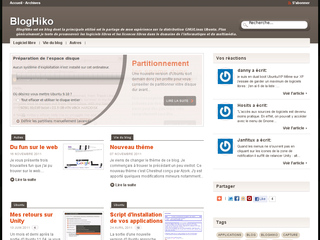
\includegraphics[width=0.5\textwidth]{./images/bloghiko.jpg}
    \caption{BlogHiko | 50\% de la largeur de la page}
\end{figure}


